\documentclass{standalone}
\usepackage{tikz}
\begin{document}
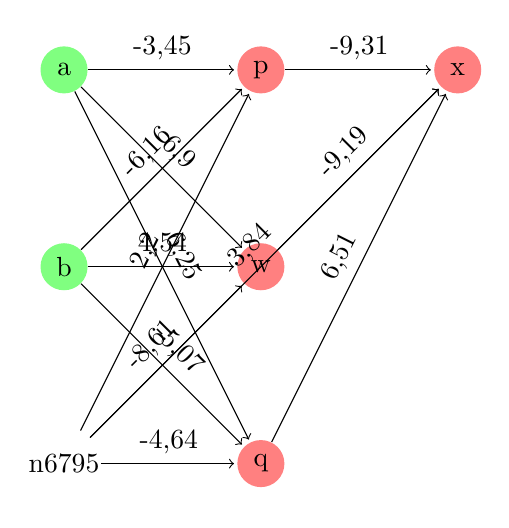
\begin{tikzpicture}[shorten >=1pt,->,draw=black!,node distance=2.5cm]
\tikzstyle{neuron}=[circle,fill=black!25,minimum size=17pt,inner sep=0pt]
\tikzstyle{constant}=[neuron, fill=white!50];
\tikzstyle{sigmoid}=[neuron, fill=red!50];
\tikzstyle{identity}=[neuron, fill=green!50];
\node [identity] (a) {a};
\node [identity,below of=a] (b) {b};
\node [constant,below of=b] (n6795) {n6795};
\node [sigmoid,right of=a] (p) {p};
\node [sigmoid,below of=p] (w) {w};
\node [sigmoid,below of=w] (q) {q};
\node [sigmoid,right of=p] (x) {x};
\path[every node/.style={sloped,anchor=south,auto=false}]
(w) edge node {-9,19} (x)
(q) edge node {6,51} (x)
(b) edge node {-5,07} (q)
(b) edge node {-6,16} (p)
(b) edge node {4,54} (w)
(n6795) edge node {-4,64} (q)
(n6795) edge node {-8,61} (w)
(n6795) edge node {2,2} (p)
(n6795) edge node {3,84} (x)
(a) edge node {6,9} (w)
(a) edge node {6,25} (q)
(a) edge node {-3,45} (p)
(p) edge node {-9,31} (x)
;\end{tikzpicture}
\end{document}